% !TEX root = sum1.tex
\section{Results}
We carried out several experiments, including comparing the running time of decomposition and Integer programming, comparing the number of people served using the feasible seat planning and Integer programming methods, analyzing different policies under the two booking situations, evaluating the results under varying demands, assessing the results for different numbers of people in each period and finally investigating the impact of seat layout on the number of served people.

\subsection{Running time of Benders Decomposition and IP}\label{Bender_IP}
% At first, we compare the running time of these two methods. 

The running times of solving DEF directly and solving the relaxation of DEF with Benders decomposition are shown in Table \ref{tab_1}.

\begin{table}[ht]
  \centering
  \caption{Running time of Decomposion and IP}\label{tab_1}
  \begin{tabular}{|l|l|l|l|l|l|l|}
  \hline
  \# of scenarios & demands & running time of IP(s) & Benders (s) & \# of rows & \# of groups & \# of seats\\
  \hline
  1000  & (150, 350) & 5.1  & 0.13 & 30 & 8 & (21, 50)\\
  5000  & & 28.73 & 0.47 & 30 & 8 \\
  10000 & & 66.81  & 0.91 & 30 & 8 \\
  50000 & & 925.17 & 4.3 & 30 & 8 \\
  \hline
  1000  & (1000, 2000) & 5.88 & 0.29 & 200 & 8 & (21, 50)\\
  5000  & & 30.0 & 0.62 & 200 & 8 \\
  10000 & & 64.41 & 1.09 & 200 & 8 \\
  50000 & & 365.57 & 4.56 & 200 & 8 \\
  \hline
  1000  & (150, 250) & 17.15  & 0.18 & 30 & 16 & (41, 60) \\
  5000  & & 105.2  & 0.67 & 30 & 16  \\
  10000 & & 260.88 & 1.28 & 30 & 16  \\
  50000 & & 3873.16 & 6.18 & 30 & 16  \\
  \hline
  \end{tabular}
\end{table}

The parameters in the columns of the table are the number of scenarios, the range of demands, running time of integer programming, running time of Benders decomposition method, the number of rows, the number of group types and the number of seats for each row, respectively. 

Take the first experiment as an example, the scenarios of demands are generated from (150, 350) randomly, the number of seats for each row is generated from (21, 50) randomly.
% about 1000 seats.

% The second one:
% The number of seats for each row L is generated from (21, 50) randomly, about 7000 seats.
% The scenarios of demands are generated from (1000, 2000) randomly.

% The third one:
% The number of seats for each row L is generated from 41-60 randomly, about 1500 seats.
% The scenarios of demands are generated from (150, 250) randomly.

\subsection{Feasible Seat Planning versus IP Solution}
An arrival sequence can be expressed as $\{y_{1}, y_{2}, \ldots, y_{T}\}$. Let $N_{i} = \sum_{t} I(y_t = i)$, i.e., the number of times group type $i$ arrives during $T$ periods. Then the scenarios, $(N_1, \ldots, N_{M})$, follow a multinomial distribution, $$p\left(N_1, \ldots, N_{M} \mid \mathbf{p}\right)=\frac{T !}{N_{1}!, \ldots, N_{M}!} \prod_{i=1}^{M} p_{i}^{N_i}, T = \sum_{i=1}^{M} N_{i}.$$

It is clear that the number of different sequences is $M^{T}$. The number of different scenarios is $O(T^{M-1})$ which can be obtained by the following DP.

Use $D(T, M) $ to denote the number of scenarios, which equals the number of different solutions to $x_{1}+\ldots + x_{M} = T, \mathbf{x} \geq 0$. Then, we know the recurrence relation $D(T, M) = \sum_{i= 0}^{T} D(i, M-1)$ and boundary condition, $D(i,1) = 1$. So we have $D(T,2) = T+1$, $D(T,3) = \frac{(T+2)(T+1)}{2}, D(T,M) = O(T^{M-1})$. The number of scenarios is too large to enumerate all possible cases. Thus, we choose to sample some sequences from the multinomial distribution.

Then, we will show the feasible seat assignment has a close performance with IP when considering group-type control policy.

\begin{table}[ht]
    \caption{Results of Feasible Seat Planning and IP solution}
    \begin{tabular}{|l|l|l|l|l|l|l|}
    \hline
    \# samples & T & probabilities & \# rows & people served by decomposition & people served by IP \\
    1000  & 45  & [0.4,0.4,0.1,0.1] & 8 & 85.30 & 85.3 \\
    1000  & 50  & [0.4,0.4,0.1,0.1] & 8 & 97.32 & 97.32 \\
    1000  & 55  & [0.4,0.4,0.1,0.1] & 8 & 102.40 & 102.40  \\ % slow
    1000  & 60  & [0.4,0.4,0.1,0.1] & 8 & 106.70 & NA  \\
    1000  & 65  & [0.4,0.4,0.1,0.1] & 8 & 108.84 & 108.84 \\
    \hline
    1000  & 35  & [0.25,0.25,0.25,0.25] & 8 & 87.16 & 87.08 \\
    1000  & 40  & [0.25,0.25,0.25,0.25] & 8 & 101.32 & 101.24 \\
    1000  & 45  & [0.25,0.25,0.25,0.25] & 8 & 110.62 & 110.52 \\
    1000  & 50  & [0.25,0.25,0.25,0.25] & 8 & 115.46 & NA \\
    1000  & 55  & [0.25,0.25,0.25,0.25] & 8 & 117.06 & 117.26 \\
    \hline
    5000  & 300  & [0.25,0.25,0.25,0.25] & 30 & 749.76 & 749.76 \\
    5000  & 350  & [0.25,0.25,0.25,0.25] & 30 & 866.02 & 866.42 \\
    5000  & 400  & [0.25,0.25,0.25,0.25] & 30 & 889.02 & 889.44 \\
    5000  & 450  & [0.25,0.25,0.25,0.25] & 30 & 916.16 & 916.66 \\
    \hline
    \end{tabular}
\end{table}

Each entry of people served is the average of 50 instances.
IP will spend more than 2 hours in some instances, as `NA' showed in the table.
The number of seats is 20 when the number of rows is 8, the number of seats is 40 when the number of rows is 30.

% We can find that the people served by Benders decomposition and IP under nested policy are close. But obtaining the near-optimal seat assignment will be faster.

% Thus, we can use the near-optimal seat assignment from the decomposition approach.

\subsection{Results of Different Policies}
In this section, we compare the performance of four dynamic seat assignment policies to the optimal value, which can be obtained by solving the deterministic model after observing all arrivals. The policies under examination are the stochastic planning policy, DP Base-heuristic, bid-price policy and FCFS policy. The seat layout consists of 10 rows, each with 21 seats (including one dummy seat), and the group size can range up to 4 people. We conducted experiments over 60 to 100 periods to demonstrate the policies' performance under varying demand levels. We selected three probabilities to ensure that the expected number of people for each period is consistent. The table below displays the average of 200 instances for each number.

\begin{table}[ht]
  \centering
  \caption{Results of different policies}
  \begin{tabular}{|l|l|l|l|l|l|}
  \hline
   T & probabilities & Sto(\%) & DP1(\%) & Bid-price(\%) & FCFS(\%) \\
  \hline
   60  & [0.25, 0.25, 0.25, 0.25]  & 99.12 & 98.42 & 98.38 & 98.17 \\
   70  & [0.25, 0.25, 0.25, 0.25]  & 98.34 & 96.87 & 96.24 & 94.75 \\
   80  & [0.25, 0.25, 0.25, 0.25]  & 98.61 & 95.69 & 96.02 & 93.18 \\
   90  & [0.25, 0.25, 0.25, 0.25]  & 99.10 & 96.05 & 96.41 & 92.48 \\
   100 & [0.25, 0.25, 0.25, 0.25]  & 99.58 & 95.09 & 96.88 & 92.54 \\
   \hline
   60  & [0.25, 0.35, 0.05, 0.35]  & 98.94 & 98.26 & 98.25 & 98.62 \\
   70  & [0.25, 0.35, 0.05, 0.35]  & 98.05 & 96.62 & 96.06 & 93.96 \\
   80  & [0.25, 0.35, 0.05, 0.35]  & 98.37 & 96.01 & 95.89 & 92.88 \\
   90  & [0.25, 0.35, 0.05, 0.35]  & 99.01 & 96.77 & 96.62 & 92.46 \\
   100 & [0.25, 0.35, 0.05, 0.35]  & 99.23 & 97.04 & 97.14 & 92.00 \\
  \hline
  60  & [0.15, 0.25, 0.55, 0.05]  & 99.14 & 98.72 & 98.74 & 98.07 \\
  70  & [0.15, 0.25, 0.55, 0.05]  & 99.30 & 96.38 & 96.90 & 96.25 \\
  80  & [0.15, 0.25, 0.55, 0.05]  & 99.59 & 97.75 & 97.87 & 95.81 \\
  90  & [0.15, 0.25, 0.55, 0.05]  & 99.53 & 98.45 & 98.69 & 95.50 \\
  100 & [0.15, 0.25, 0.55, 0.05]  & 99.47 & 98.62 & 98.94 & 95.25 \\
  \hline
  \end{tabular}
\end{table}

We can find that the stochastic planning policy are better than DP Base-heuristic and bid-price policy consistently, and FCFS policy works worst. As we mentioned previously, DP Base-heuristic and bid-price policy can only make the decision to accept or deny, cannot decide which row to assign the group to. FCFS accepts groups in sequential order until the capacity cannot accommodate more.


For the first three policies, their performance tends to initially drop and then increase as the number of periods increases. When the number of periods is small, the demand for capacity is relatively low, and the policies can achieve relatively optimal performance. However, as the number of periods increases, the policies may struggle to always obtain a perfect allocation plan, leading to a decrease in performance. Nevertheless, when the number of periods continue to become larger, these policies tend to accept larger groups, and as a result, narrow the gap with the optimal value, leading to an increase in performance.

%  当之前的上座率 小于 gamma/gamma+1, 制定社交距离没有影响
%  大于 gamma/gamma+1, 则最大损失是(  )

\subsection{Impact of Social Distance under Different Demands}
In this section, we will explore how social distancing affects the occupancy rate of a venue under different demands. Let $\gamma$ represent the average number of people who arrive in each period, and let $L$ represent the total number of seats available. We can calculate the expected number of people arriving using the formula $E(D) = \gamma T$, where $T$ is the number of periods. 

If we assume that we accept all incoming groups within the $T{'}$ periods and they fill all the available seats, then we have $E(D) + T{'} = L$. Solving for $T{'}$, we get $T{'} = L/(\gamma + 1)$. 
$T{'}$ represents the ideal first period where the number of people without social distancing is larger than that with social distancing and the gap percentage is the corresponding percentage of total seats. But the actual first period will be smaller than the ideal one because we cannot always exactly fill the seats with accepted groups. 


If we limit the number of group types to 4, we can express $\gamma$ as $\gamma = p_1 * 1 + p_2 * 2 + p_3 * 3 + p_4 * 4$, where $p_1$, $p_2$, $p_3$, and $p_4$ represent the probabilities of groups with one, two, three, and four people, respectively. Define each combination $(p_1, p_2, p_3, p_4)$ such that $p_1 + p_2 + p_3 + p_4 = 1$ as a probability combination. Specifically, we consider two situations: $\gamma = 2.5$ and $\gamma = 1.9$. When $\gamma = 2.5$, we set the parameters as follows: $T$ varies from 10 to 100, the step size is 1. When $\gamma = 1.9$, we set the parameters as follows: $T$ varies from 30 to 120, the step size is 1. The seat layout consists 10 rows and the number of seats per row is 21.

For each $\gamma$, we give several probabilities in the table. We can find the actual gap points with the same $\gamma$ are close.

\begin{table}[ht]
  \centering
  \caption{Actual Gap points of different probabilities}
  \begin{tabular}{|l|l|l|l|}
  \hline
  $\gamma$  & probabilities & gap point & gap percentage \\
  \hline
  2.5  & [0.25,0.25,0.25,0.25] & 56 & 65.21 \\
  2.5  & [0.1,0.4,0.4,0.1] & 55 & 65.59 \\
  2.5  & [0.1, 0.5, 0.2, 0.2] & 55 & 65.45 \\
  2.5  & [0.2, 0.3, 0.3, 0.2] & 54 & 64.56 \\
  2.5  & [0.3, 0.2, 0.2, 0.3] & 55 & 65.51\\
  2.5  & [0.2, 0.4, 0.1, 0.3] & 55 & 65.41 \\
  1.9  & [0.4, 0.4, 0.1, 0.1] & 67 & 60.35 \\
  1.9  & [0.5, 0.2, 0.2, 0.1] & 67 & 58.9  \\
  1.9  & [0.3, 0.5, 0.2, 0]  &  68 & 61.7  \\
  1.9  & [0.6, 0.1, 0.1, 0.2] & 66 & 58.31 \\
  \hline
  \end{tabular}
\end{table}


The figure below displays the outcomes of groups who were accepted under two different conditions: with social distancing measures and without social distancing measures. For the former case, we employ stochastic planning to obtain the results. For the latter case, we utilize a deterministic model with hindsight to generate the outcomes. Since the various probabilities with the same $\gamma$ exhibit similar patterns as shown in the figure, we present only one case of probabilities to illustrate the detailed figure.

\begin{figure}[h]
  \centering
  \subfigure[When $\gamma =2.5$]{
    \label{Fig.sub.1}
    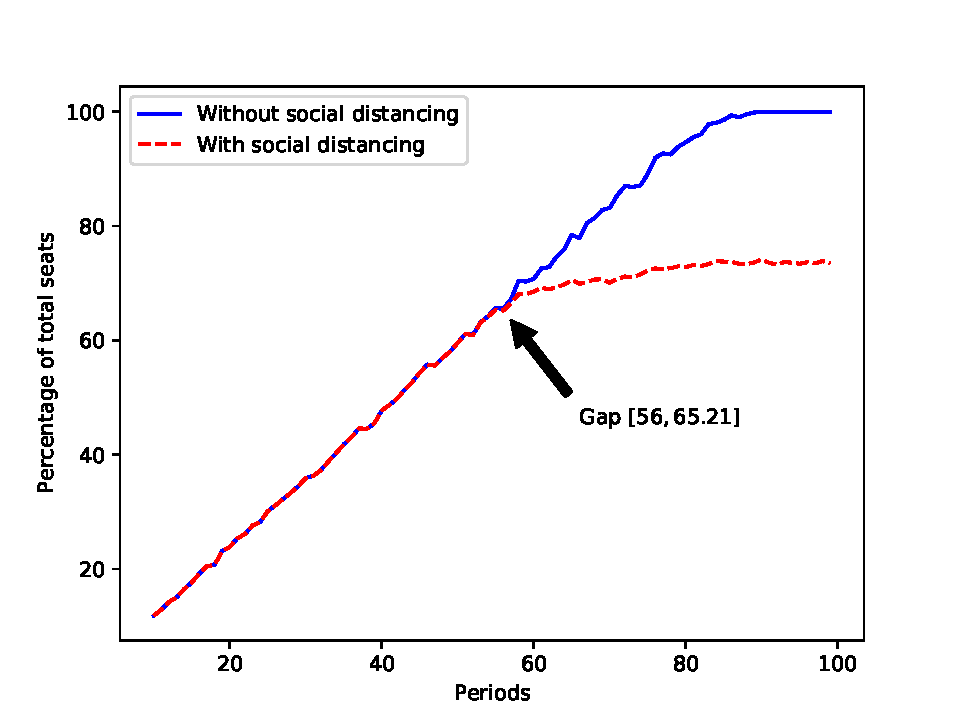
\includegraphics[width=0.48\textwidth]{./Figures/p1.pdf}}
  \subfigure[When $\gamma =1.9$]{
    \label{Fig.sub.2}
    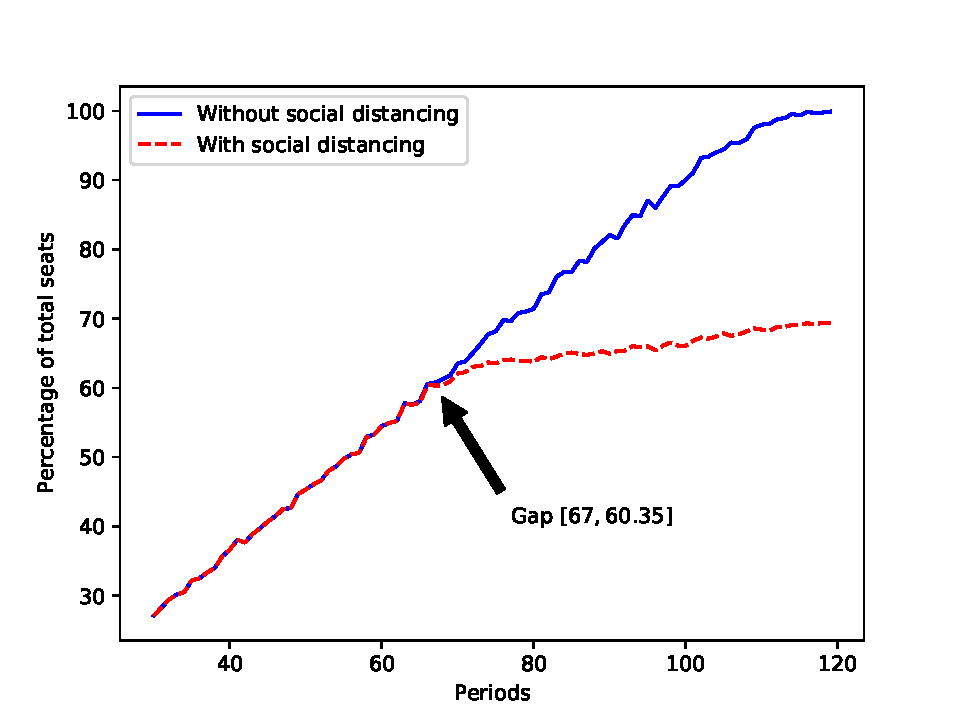
\includegraphics[width=0.48\textwidth]{./Figures/p2.pdf}}
  \caption{The number of people served versus periods}
  \label{Fig.lable}
\end{figure}


The analysis comprises three stages. In the first stage, where the capacity is sufficient, social distancing measures have no impact on the outcome. In the second stage, the gap between the outcomes with and without social distancing measures widens as $T$ increases. Finally, in the third stage, as $T$ continues to increase, the gap between the outcomes with and without social distancing measures converges when both situations accept the maximum number of people.

\begin{table}[ht]
  \centering
  \caption{Gap points and gap percentage of different probabilities}
  \begin{tabular}{|l|l|l|}
  \hline
  $\gamma$  & gap point & gap percentage \\
  \hline
  $[1.5,1.7]$   & [56, ] & [65.21, ] \\
  $[1.7,1.9]$   & [56, ] & [65.21, ] \\
  $[1.9,2.1]$   & [56, ] & [65.21, ] \\
  $[2.1,2.3]$   & [56, ] & [65.21, ] \\
  $[2.1,2.3]$   & [56, ] & [65.21, ] \\
  $[2.3,2.5]$   & [    ] & [] \\
  $[2.5,2.7]$   & [    ] & [] \\
  $[2.9,3.1]$   & [    ] & [] \\
  $[3.1,3.3]$   & [    ] & [] \\
  \hline
  \end{tabular}
\end{table}

\subsection{Comparison of Different Probabilities When Supply and Demand Are Close}
When we set the number of periods $T$ to be equal to $T'$, representing a state where the expected demand and supply are in balance, we can observe differences among the outcomes for different probabilities. In this case, the estimated occupancy rate is given by $\frac{\gamma T'}{(\gamma+1)T' - N}$. It is important to note that this estimation is accurate only when all rows represent full patterns, as per our assumption.

We sample $p_1$, $p_2$, and $p_3$ from 0.05 to 0.95 with an increment of 0.05. The seat layout still remains the same as the above experiments. The figure below shows the number of people served for each value of $\gamma$. For each probability combination, the blue point represents the average number of people served over 50 instances, and the red point represents the estimated number of people served. 

\begin{figure}[h]
  \centering
  \subfigure[One instance for each probability combination]{
    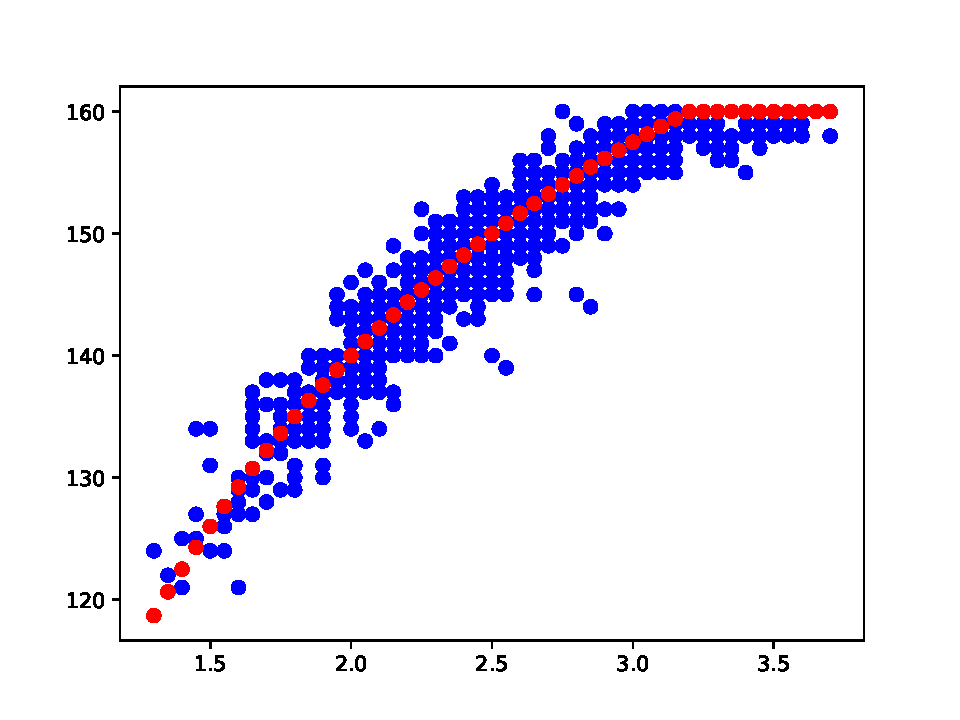
\includegraphics[width=0.48\textwidth]{./Figures/diff_1.pdf}}
  \subfigure[Average of 50 instances for each probability combination]{
    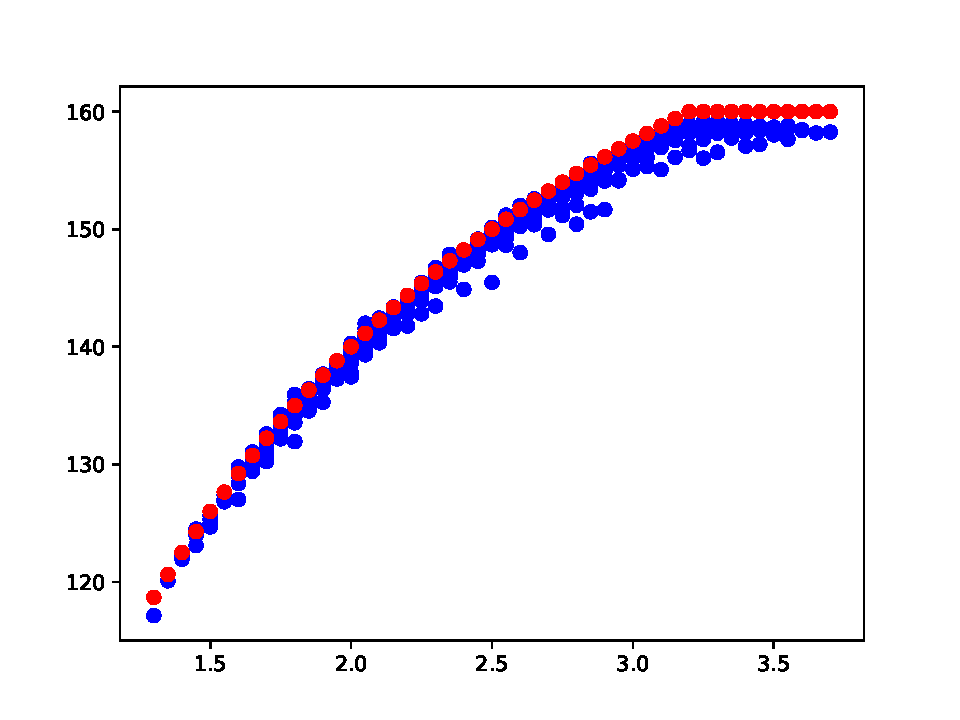
\includegraphics[width=0.48\textwidth]{./Figures/diff_2.pdf}}
  \caption{The number of people accepted versus $\gamma$}
\end{figure}

If the largest pattern is assigned to each row, the resulting occupancy rate is $\frac{16}{21}$. The maximum number of people that can be accepted is $200 * \frac{16}{20} = 160$, which is the upper bound on the number of people that can be accepted. The estimated number of people accepted is given by $\frac{\gamma}{\gamma+1} * 200$, as indicated by the red points in the figure.

\subsubsection{Analysis on The Difference Between Blue and Red Points}
We can give the absolute difference between the blue point and red point for each probability combination as below.

\begin{table}[ht]
  \centering
  \caption{Absolute Difference Proportion}\label{tab_diff}
  \begin{tabular}{|l|l|l|l|l|}
  \hline
  \# of instances & abs\_diff $\geq$ 1 & abs\_diff $\geq$ 2 & abs\_diff $\geq$ 3 & abs\_diff $\geq$ 4 \\
  \hline
  20 & 32.92 \% & 5.13 \% & 1.74\% & 0.51 \% \\
  50 & 22.46 \% & 4.31 \% & 1.54 \% & 0.31 \%  \\
  100 & 20.00 \% & 4.21 \% & 1.54 \% & 0.31 \% \\
  \hline
  \end{tabular}
\end{table}

\begin{figure}[ht]
  \centering
  \subfigure[Average of 50 instances for each probability combination]{
    \label{Fig1}
    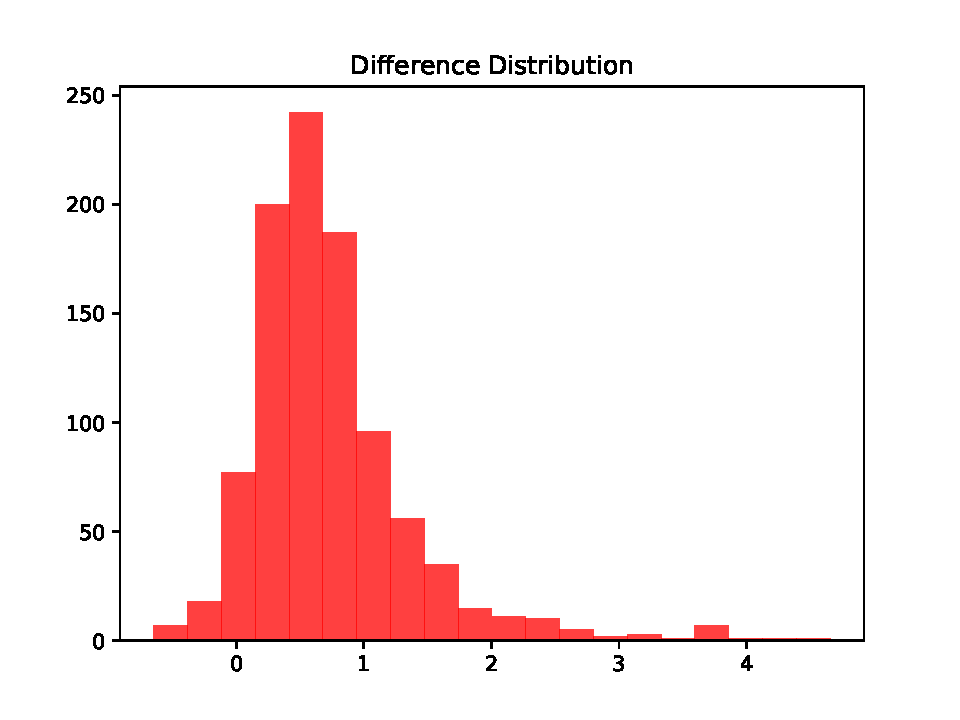
\includegraphics[width=0.48\textwidth]{./Figures/Figure_50.pdf}}
  \subfigure[Average of 100 instances for each probability combination]{
    \label{Fig2}
    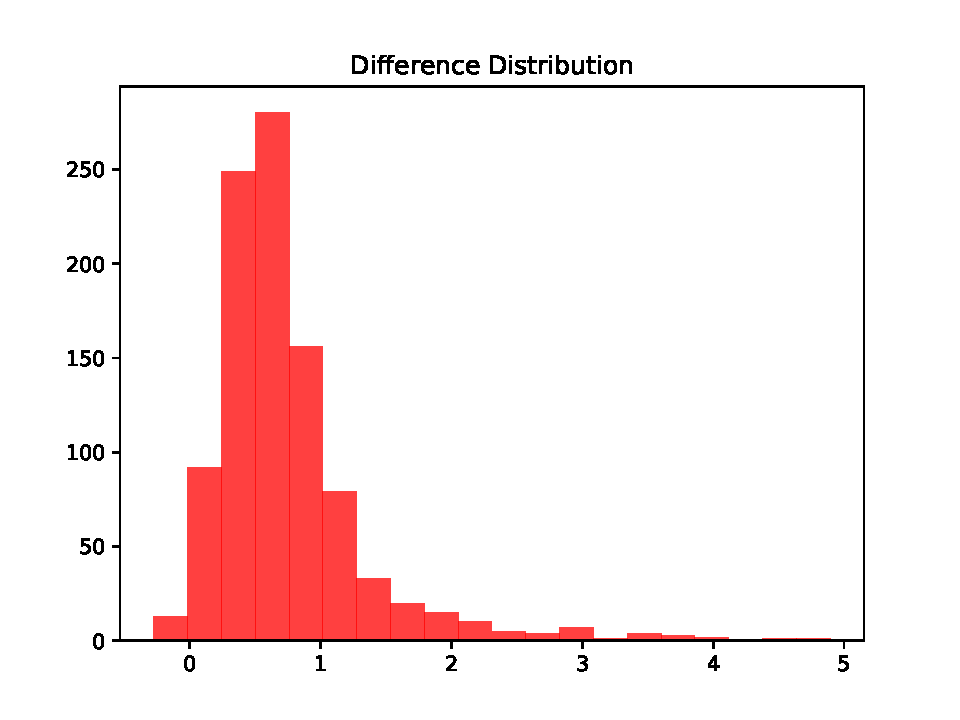
\includegraphics[width=0.48\textwidth]{./Figures/Figure_100.pdf}}
  \caption{The difference distribution}
  \label{fig_diff}
\end{figure}

Table \ref{tab_diff} displays the absolute difference proportion for the average of 20, 50, and 100 instances, while Figure \ref{fig_diff} shows the difference distribution for the average of 50 and 100 instances. These results suggest that we can estimate the attendance rate based on $\gamma$ for most probability combinations.

However, we have also observed that some blue points in the figure are significantly distant from their corresponding red points. This is evident when the probability combination is $[0.05, 0.05, 0.85, 0.05]$ (which corresponds to $\gamma = 2.9$), and the demands cannot be accommodated by constructing full patterns for every row, which does not satisfy our assumption. This leads to a considerable gap between the blue and red points in this case. For example, the demands could be $[4, 1, 45, 2]$ or $[2, 2, 47, 1]$ according to the probability combination, but the typical pattern that can be generated is $(4,4,4,4)$, which is not full.

\subsubsection{Results of Different Seat Layouts}
If we modify the even seat layout, the differences between the red and blue points will decrease, and some outliers may be eliminated. To maintain the same total seating capacity, we compare two layouts with the even seat layout. The step-size seat layout consists of rows with 17, 18, 19, 20, 21, 21, 22, 23, 24, and 25 seats, while the random seat layout has rows with 19, 20, 21, 21, 23, 24, 26, 17, 19, and 20 seats. Both layouts can accommodate a maximum of 164 people when each row corresponds to the largest pattern.

\begin{figure}[ht]
  \centering
  \subfigure[Average of 50 instances for step-size seat layout]{
    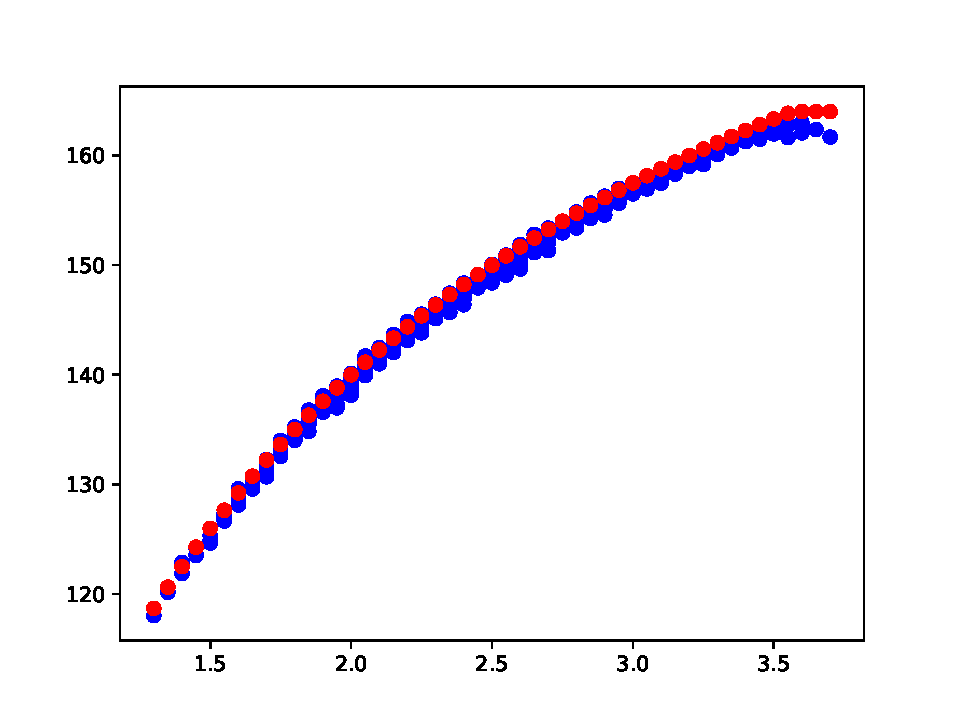
\includegraphics[width=0.48\textwidth]{./Figures/stepsize_seat.pdf}}
  \subfigure[Average of 50 instances for random seat layout]{
    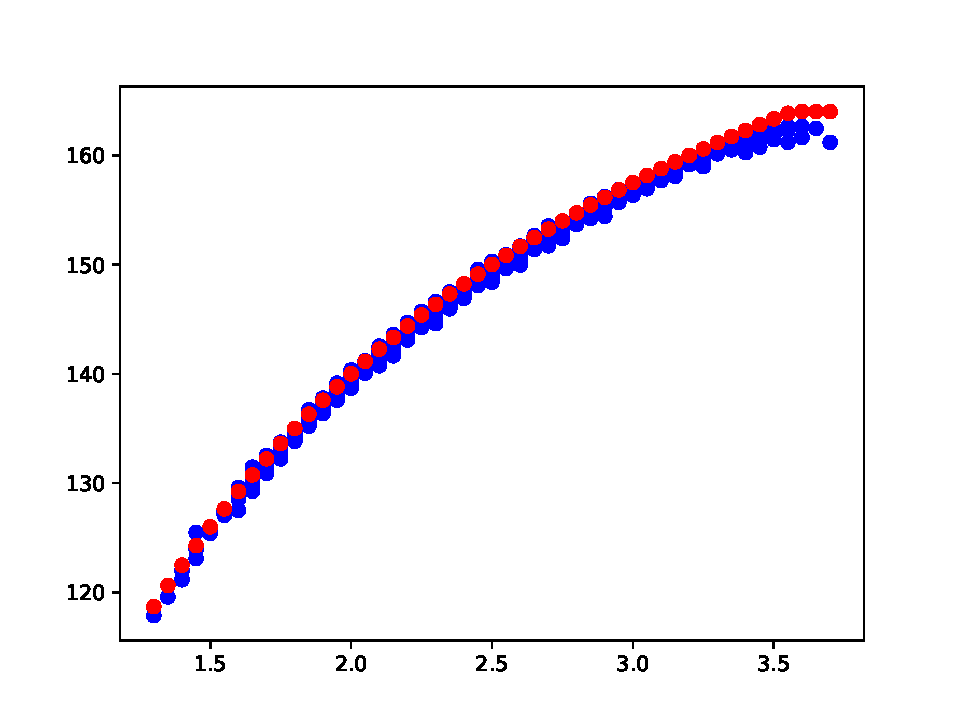
\includegraphics[width=0.48\textwidth]{./Figures/random_seat.pdf}}
  \caption{The number of people served versus $\gamma$}
\end{figure}

The results suggest that a random seat layout may provide a more accurate estimation, implying that such a layout is more capable of accommodating uncertain demands and achieving a full pattern that can accept more people.

% When $p = [0.25, 0.25, 0.25, 0.25]$, $E(D) = 2.5 T$. Let $p_1*1 + p_2*2 + p_3*3 + p_4*4 = 2.5$, 
% Let $E(D) = 150, T = 50, 60, 75$. The number of seats: 200, 210, 225.


\newpage

% In addition, we evaluate two policies for seat assignment after all group arrivals: one is based on dynamic programming (DP) and the other is based on first-come, first-served (FCFS) scheduling.
% We present the results of our experiments and discuss their implications.


% \subsection{Measurement}
% Suppose a real scenario with a fixed sequence, $s^{r}$. Solving the following program can obtain the optimal value, $V_{s^{r}}$. (Offline)

% Then the difference is $V_{s^{r}} - \text{our result}$.

% WS(the value under wait-and-see policy with all possible scenarios)

% EVPI(Expected Value of Perfect Information) = WS - the value of deterministic equivalent form
